% =============================================================================
% ΚΕΦΑΛΑΙΟ 5: ΑΠΟΤΕΛΕΣΜΑΤΑ ΚΑΙ ΑΞΙΟΛΟΓΗΣΗ
% =============================================================================
% Τα αριθμητικά αποτελέσματα προέρχονται από τους πίνακες
% simulations.energy_prices (code_version 9, μέθοδος merit_order) και
% entsoe.energy_prices της βάσης δεδομένων του συστήματος. Τα σχήματα
% παρήχθησαν από τα ίδια δεδομένα (figures/gr_*.pdf).
% =============================================================================

\chapter{Αποτελέσματα και Αξιολόγηση}
\label{ch:results}

Στο παρόν κεφάλαιο παρουσιάζονται τα αποτελέσματα της εφαρμογής του συστήματος προσομοίωσης και η αξιολόγησή τους μέσω σύγκρισης με τις πραγματικές τιμές της Προημερήσιας Αγοράς. Το κεντρικό εύρημα είναι ότι το βιβλίο εντολών οριακού κόστους (merit-order order book, Ενότητα~\ref{sec:merit-order-book}) με τους κύριους θεμελιώδεις παράγοντες της αγοράς --- πραγματικές τιμές φυσικού αερίου TTF, ημερήσιες τιμές δικαιωμάτων CO$_2$, αξία νερού συναρτήσει της πληρότητας των ταμιευτήρων, αυτοπρογραμματισμός μονάδων βάσης, και παρατηρούμενες καθαρές εισαγωγές --- αναπαράγει τις τιμές εκκαθάρισης της ελληνικής ζώνης με \textbf{συνολικό συντελεστή συσχέτισης $r = 0{,}84$} σε τετράμηνη περίοδο συνεχούς προσομοίωσης δεκαπενταλέπτου, με πρακτικά μηδενική συστηματική απόκλιση ($-2{,}5$~€/MWh). Η ανάλυση περιλαμβάνει τη μεθοδολογία επικύρωσης, τη στατιστική σύγκριση τιμών, την ανάλυση της συνεισφοράς των επιμέρους παραγόντων του μοντέλου, την πολυζωνική αξιολόγηση, και την υπολογιστική απόδοση. Τέλος, συζητούνται οι περιορισμοί της προσέγγισης και οι πηγές απόκλισης από τις πραγματικές τιμές.


% =============================================================================
\section{Μεθοδολογία Επικύρωσης}
\label{sec:validation-methodology}

Η επικύρωση βασίζεται στη σύγκριση των υπολογισμένων τιμών εκκαθάρισης με τις πραγματικές τιμές που δημοσιεύονται στην πλατφόρμα διαφάνειας του ENTSO-E. Χρησιμοποιούνται δύο συμπληρωματικά σύνολα δεδομένων: μια συνεχής περίοδος τεσσάρων μηνών για τη συνολική αξιολόγηση, και ένα σταθερό, εκτός δείγματος (held-out) σύνολο ημερών διασποράς τριών ετών, το οποίο δεν χρησιμοποιήθηκε ποτέ για ρύθμιση παραμέτρων.

\subsection{Σύνολα Δεδομένων Επικύρωσης}
\label{subsec:validation-dataset}

Το κύριο σύνολο επικύρωσης καλύπτει τη συνεχή περίοδο από 1 Μαρτίου έως 30 Ιουνίου 2026 για την ελληνική ζώνη προσφοράς, στη φυσική χρονική ανάλυση της αγοράς (δεκαπενταλεπτα διαστήματα εμπορίας, τα οποία εισήχθησαν στην ελληνική Προημερήσια Αγορά τον Οκτώβριο του 2025). Ο Πίνακας~\ref{tab:validation-dataset} συνοψίζει τα χαρακτηριστικά του.

\begin{table}[htbp]
\centering
\caption{Χαρακτηριστικά κύριου συνόλου δεδομένων επικύρωσης}
\label{tab:validation-dataset}
\begin{tabular}{@{}ll@{}}
\toprule
\textbf{Παράμετρος} & \textbf{Τιμή} \\
\midrule
Περίοδος αναφοράς & 1/3/2026 -- 30/6/2026 \\
Αριθμός ημερών & 122 \\
Χρονική ανάλυση & 15 λεπτά (96 διαστήματα/ημέρα) \\
Συνολικές παρατηρήσεις & 11.712 \\
Ζώνη προσφοράς & GR (μονοζωνική εκκαθάριση) \\
Πολυζωνική εκκαθάριση & GR, BG, RO, RS, HU (ωριαία) \\
Μέση πραγματική τιμή & 91,5 €/MWh \\
Μέθοδος & merit-order βιβλίο εντολών, MPCC \\
\bottomrule
\end{tabular}
\end{table}

Συμπληρωματικά, διατηρείται ένα σταθερό σύνολο 24 ημερών επικύρωσης εκτός δείγματος, επιλεγμένων με ψευδοτυχαία δειγματοληψία από την περίοδο 2023--2026 ώστε να καλύπτουν όλες τις εποχές και διαφορετικά καθεστώτα τιμών (συμπεριλαμβανομένων ημερών ξηρασίας και περιφερειακής σύζευξης με υψηλές τιμές). Το σύνολο αυτό χρησιμοποιείται αποκλειστικά για αξιολόγηση: καμία παράμετρος του μοντέλου δεν ρυθμίστηκε με βάση τις ημέρες αυτές, ώστε οι μετρικές να αποτυπώνουν την ικανότητα γενίκευσης και όχι υπερπροσαρμογή.

\subsection{Μετρικές Αξιολόγησης}
\label{subsec:evaluation-metrics}

Για την ποσοτική αξιολόγηση χρησιμοποιούνται οι ακόλουθες στατιστικές μετρικές:

\paragraph{Μέσο Απόλυτο Σφάλμα (Mean Absolute Error - MAE)}
\begin{equation}
\text{MAE} = \frac{1}{n} \sum_{i=1}^{n} |p_i^{\text{calc}} - p_i^{\text{actual}}|
\label{eq:mae}
\end{equation}
όπου $p_i^{\text{calc}}$ είναι η υπολογισμένη τιμή και $p_i^{\text{actual}}$ η πραγματική τιμή για την παρατήρηση $i$.

\paragraph{Ρίζα Μέσου Τετραγωνικού Σφάλματος (Root Mean Square Error - RMSE)}
\begin{equation}
\text{RMSE} = \sqrt{\frac{1}{n} \sum_{i=1}^{n} (p_i^{\text{calc}} - p_i^{\text{actual}})^2}
\label{eq:rmse}
\end{equation}

\paragraph{Συστηματική Απόκλιση (bias)}
\begin{equation}
\text{bias} = \frac{1}{n} \sum_{i=1}^{n} (p_i^{\text{calc}} - p_i^{\text{actual}})
\label{eq:bias}
\end{equation}

\paragraph{Συντελεστής Συσχέτισης Pearson}
\begin{equation}
r = \frac{\sum_{i=1}^{n}(p_i^{\text{calc}} - \bar{p}^{\text{calc}})(p_i^{\text{actual}} - \bar{p}^{\text{actual}})}{\sqrt{\sum_{i=1}^{n}(p_i^{\text{calc}} - \bar{p}^{\text{calc}})^2 \sum_{i=1}^{n}(p_i^{\text{actual}} - \bar{p}^{\text{actual}})^2}}
\label{eq:pearson}
\end{equation}

\paragraph{Συντελεστής Προσδιορισμού ($R^2$)}
Ο $R^2$ υπολογίζεται ως προς την ταυτοτική πρόβλεψη $y=x$ (όχι ως προς την ευθεία ελαχίστων τετραγώνων), ώστε να τιμωρεί και τη συστηματική απόκλιση:
\begin{equation}
R^2 = 1 - \frac{\sum_{i=1}^{n}(p_i^{\text{actual}} - p_i^{\text{calc}})^2}{\sum_{i=1}^{n}(p_i^{\text{actual}} - \bar{p}^{\text{actual}})^2}
\label{eq:r-squared}
\end{equation}

Το Μέσο Απόλυτο Ποσοστιαίο Σφάλμα (MAPE) \emph{δεν} αναφέρεται, διότι στην εξεταζόμενη περίοδο οι πραγματικές τιμές λαμβάνουν συστηματικά τιμές πλησίον του μηδενός τις μεσημβρινές ώρες υψηλής φωτοβολταϊκής παραγωγής (βλ. Σχήμα~\ref{fig:gr-intraday-profile}), γεγονός που καθιστά τον παρονομαστή της μετρικής παθολογικό. Αντ' αυτού αναφέρεται το σχετικό MAE ως προς τη μέση πραγματική τιμή.

\subsection{Διαδικασία Σύγκρισης}
\label{subsec:comparison-procedure}

Η προσομοίωση εκτελείται για κάθε ημέρα της περιόδου με τις πληροφορίες που ήταν διαθέσιμες κατά τον χρόνο της δημοπρασίας (προημερήσιες προβλέψεις φορτίου και ΑΠΕ, τιμή κλεισίματος TTF και EUA της προηγούμενης ημέρας διαπραγμάτευσης --- αυστηρά χωρίς πληροφορία από το μέλλον), και οι υπολογισμένες τιμές αποθηκεύονται στον πίνακα \texttt{simulations.energy\_prices} με αναγνωριστικό έκδοσης μοντέλου (\texttt{code\_version}). Οι πραγματικές τιμές ανακτώνται από τον πίνακα \texttt{entsoe.energy\_prices}, οι χρονοσειρές ευθυγραμμίζονται ανά ζώνη και δεκαπεντάλεπτο σε UTC, και υπολογίζονται οι μετρικές. Τα αποτελέσματα κάθε έκδοσης του μοντέλου παραμένουν διαθέσιμα στη βάση, ώστε η εξέλιξη της ακρίβειας μεταξύ διαδοχικών εκδόσεων να είναι πλήρως αναπαραγώγιμη και εποπτεύσιμη μέσω διαδραστικού πίνακα οργάνων (Metabase).


% =============================================================================
\section{Αποτελέσματα για την Ελληνική Ζώνη}
\label{sec:price-comparison}

\subsection{Συνολικές Μετρικές}
\label{subsec:gr-results}

Ο Πίνακας~\ref{tab:gr-metrics} συνοψίζει τις μετρικές για το κύριο σύνολο επικύρωσης (122 ημέρες, 11.712 δεκαπεντάλεπτα).

\begin{table}[htbp]
\centering
\caption{Μετρικές αξιολόγησης για τη ζώνη της Ελλάδας (GR), 1/3--30/6/2026, ανάλυση 15 λεπτών}
\label{tab:gr-metrics}
\begin{tabular}{@{}lc@{}}
\toprule
\textbf{Μετρική} & \textbf{Τιμή} \\
\midrule
MAE (€/MWh) & 27,2 \\
Σχετικό MAE (\% της μέσης τιμής) & 29,7 \\
RMSE (€/MWh) & 38,4 \\
Συντελεστής Pearson ($r$) & \textbf{0,844} \\
$R^2$ (ως προς $y=x$) & 0,637 \\
\midrule
Μέση υπολογισμένη τιμή (€/MWh) & 89,0 \\
Μέση πραγματική τιμή (€/MWh) & 91,5 \\
Συστηματική απόκλιση (bias, €/MWh) & $-2{,}5$ \\
\bottomrule
\end{tabular}
\end{table}

Τρία σημεία αξίζουν έμφασης. Πρώτον, ο συντελεστής συσχέτισης $r=0{,}844$ επιτυγχάνεται σε ανάλυση δεκαπενταλέπτου και σε συνεχή τετράμηνη περίοδο --- δεν πρόκειται για επιλεγμένες ημέρες. Δεύτερον, η συστηματική απόκλιση είναι πρακτικά μηδενική ($-2{,}5$~€/MWh, δηλαδή 2{,}7\% της μέσης τιμής): το μοντέλο δεν υπερεκτιμά ούτε υποεκτιμά συστηματικά το επίπεδο των τιμών. Τρίτον, η διαφορά μεταξύ MAE και RMSE υποδεικνύει ότι το σφάλμα συγκεντρώνεται σε λίγες ακραίες ώρες· η διάμεση ημέρα προσομοιώνεται σημαντικά καλύτερα από ό,τι δηλώνει ο μέσος όρος.

Το Σχήμα~\ref{fig:gr-price-timeseries} παρουσιάζει τις μέσες ημερήσιες τιμές των δύο χρονοσειρών για ολόκληρη την περίοδο, και το Σχήμα~\ref{fig:gr-week-timeseries} μια αντιπροσωπευτική εβδομάδα σε πλήρη ανάλυση δεκαπενταλέπτου, όπου διακρίνεται η ικανότητα του μοντέλου να αναπαράγει τόσο τη μεσημβρινή κατάρρευση των τιμών λόγω φωτοβολταϊκών όσο και τις βραδινές αιχμές.

\begin{figure}[htbp]
\centering
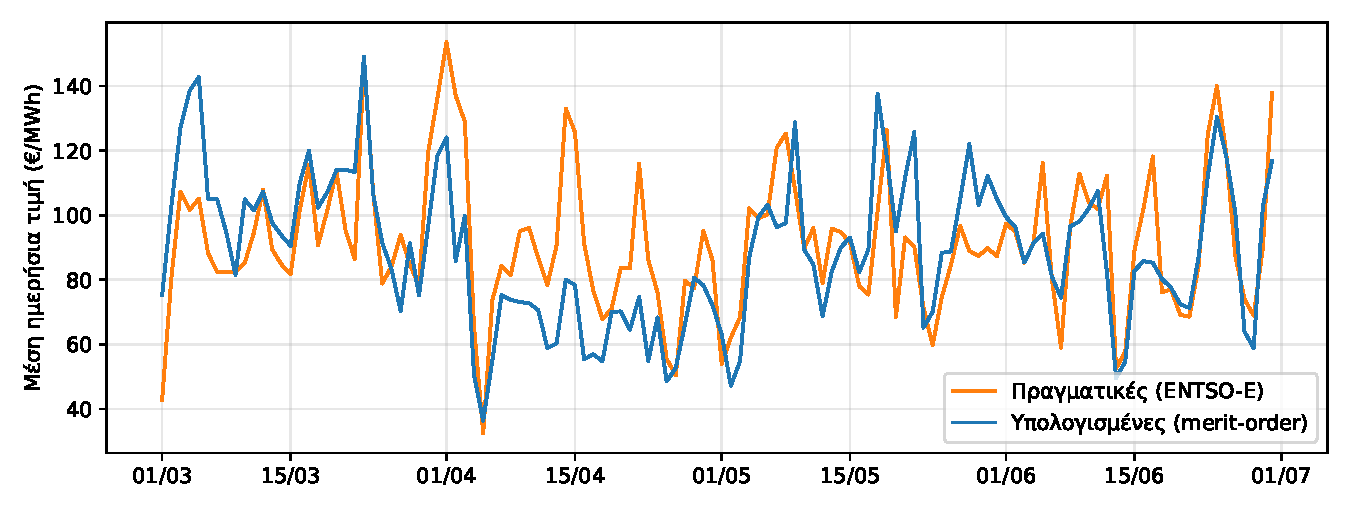
\includegraphics[width=\textwidth]{figures/gr_daily_timeseries.pdf}
\caption{Μέσες ημερήσιες τιμές: υπολογισμένες έναντι πραγματικών για τη ζώνη GR, 1/3--30/6/2026.}
\label{fig:gr-price-timeseries}
\end{figure}

\begin{figure}[htbp]
\centering
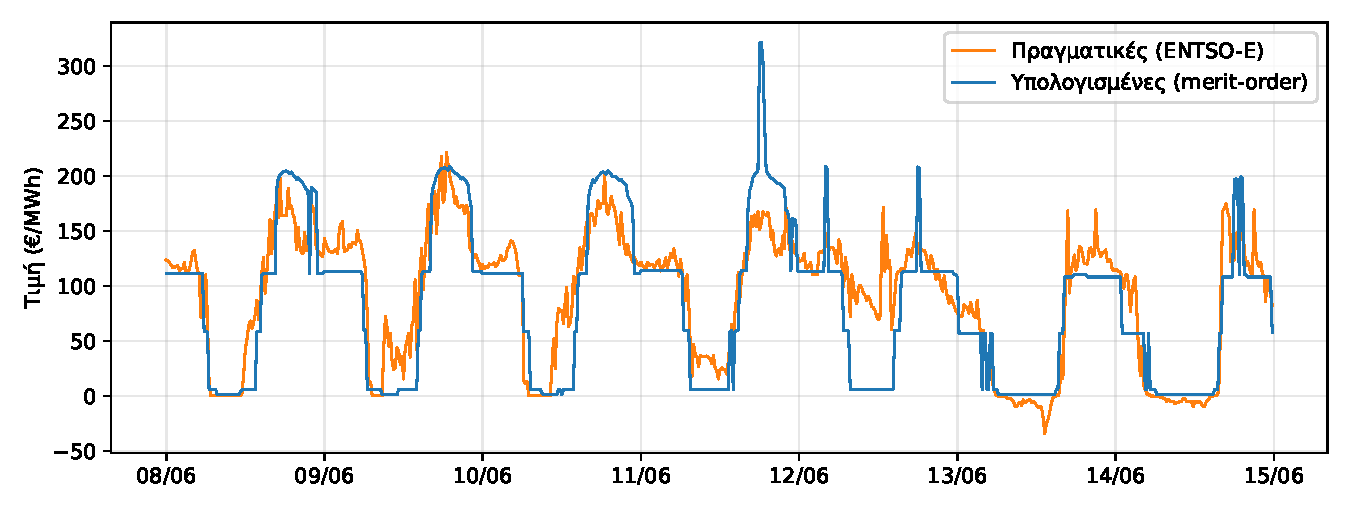
\includegraphics[width=\textwidth]{figures/gr_week_timeseries.pdf}
\caption{Υπολογισμένες και πραγματικές τιμές σε ανάλυση 15 λεπτών για την εβδομάδα 8--14/6/2026.}
\label{fig:gr-week-timeseries}
\end{figure}

Το διάγραμμα διασποράς (Σχήμα~\ref{fig:gr-scatter}) απεικονίζει τη σχέση μεταξύ υπολογισμένων και πραγματικών τιμών σε επίπεδο δεκαπενταλέπτου, με την ευθεία $y=x$ να αντιπροσωπεύει την τέλεια συμφωνία.

\begin{figure}[htbp]
\centering
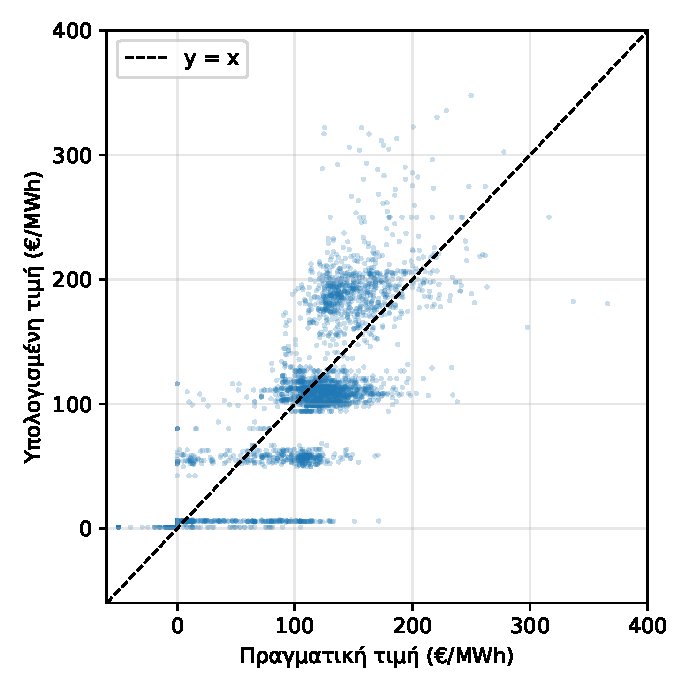
\includegraphics[width=0.62\textwidth]{figures/gr_scatter.pdf}
\caption{Διάγραμμα διασποράς υπολογισμένων έναντι πραγματικών τιμών (τυχαίο δείγμα 4.000 δεκαπενταλέπτων).}
\label{fig:gr-scatter}
\end{figure}

\subsection{Ενδοημερήσια Δομή}
\label{subsec:hourly-analysis}

Πέρα από το συνολικό επίπεδο, κρίσιμο ερώτημα είναι αν το μοντέλο αναπαράγει το ενδοημερήσιο \emph{σχήμα} των τιμών --- την «καμπύλη πάπιας» με τη μεσημβρινή βύθιση λόγω φωτοβολταϊκών και τις πρωινές/βραδινές αιχμές. Το Σχήμα~\ref{fig:gr-intraday-profile} συγκρίνει το μέσο ενδοημερήσιο προφίλ των δύο χρονοσειρών σε όλη την περίοδο: η βύθιση, τα σημεία καμπής της (που καθορίζονται από την ανατολή και δύση του ηλίου μέσω των προβλέψεων ΑΠΕ), και οι αιχμές ευθυγραμμίζονται χρονικά.

\begin{figure}[htbp]
\centering
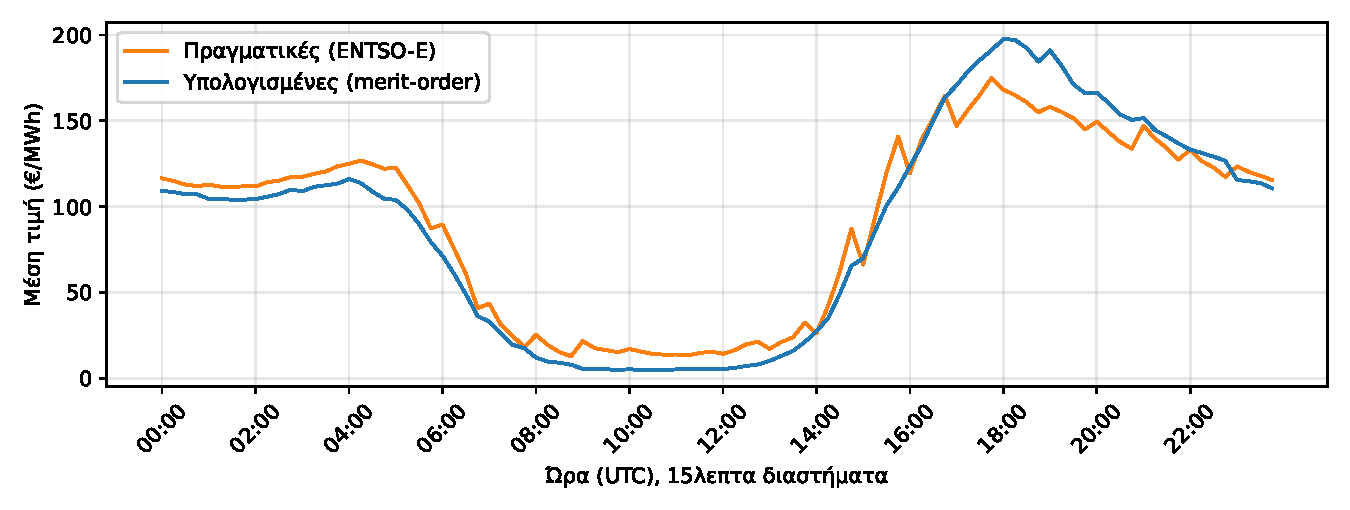
\includegraphics[width=\textwidth]{figures/gr_intraday_profile.pdf}
\caption{Μέσο ενδοημερήσιο προφίλ τιμών (96 δεκαπεντάλεπτα), μέσος όρος 122 ημερών.}
\label{fig:gr-intraday-profile}
\end{figure}

Για την ποσοτικοποίηση, υπολογίζεται ο συντελεστής συσχέτισης \emph{εντός κάθε ημέρας} ξεχωριστά (96 σημεία ανά ημέρα), ο οποίος είναι αναλλοίωτος στο ημερήσιο επίπεδο τιμών και μετρά αποκλειστικά το σχήμα. Η κατανομή του παρουσιάζεται στο Σχήμα~\ref{fig:gr-daycorr-hist}: μέση τιμή 0,876, διάμεσος \textbf{0,898}, με 96 από τις 122 ημέρες (79\%) να υπερβαίνουν το 0,85 και 113 (93\%) το 0,70. Αντίθετα, η συσχέτιση των \emph{ημερήσιων μέσων} τιμών είναι 0,66: το μοντέλο αναπαράγει το ενδοημερήσιο σχήμα ισχυρότερα από το ημερήσιο επίπεδο, το οποίο εξαρτάται από παράγοντες (π.χ. συμπεριφορά προσφορών σε ημέρες στενότητας) που δεν αποτυπώνονται πλήρως στο ανταγωνιστικό μοντέλο (βλ. Ενότητα~\ref{sec:results-limitations}).

\begin{figure}[htbp]
\centering
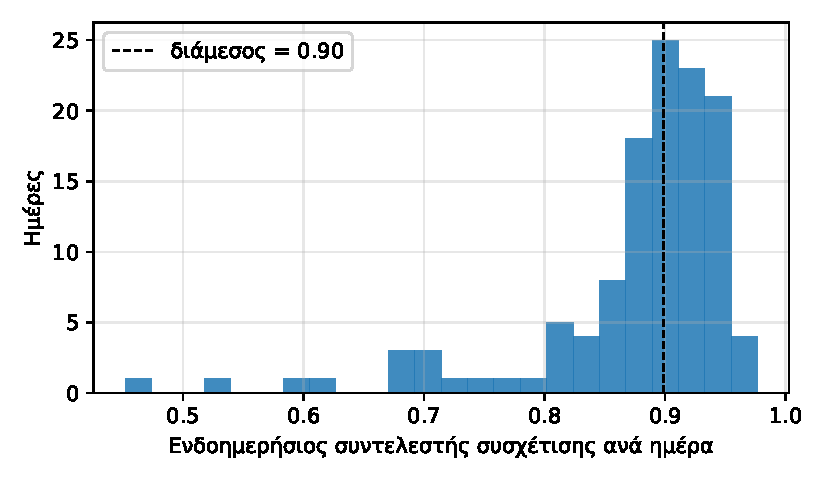
\includegraphics[width=0.7\textwidth]{figures/gr_daycorr_hist.pdf}
\caption{Κατανομή του ενδοημερήσιου συντελεστή συσχέτισης ανά ημέρα (122 ημέρες).}
\label{fig:gr-daycorr-hist}
\end{figure}

\subsection{Επίδοση σε Σύνολο Εκτός Δείγματος}
\label{subsec:heldout-results}

Στο σταθερό σύνολο των 24 ημερών εκτός δείγματος (2023--2026, όλες οι εποχές, συμπεριλαμβανομένων ακραίων ημερών ξηρασίας και περιφερειακής στενότητας), το μοντέλο επιτυγχάνει MAE 31,4~€/MWh, RMSE 41,8~€/MWh, μέση ημερήσια συσχέτιση 0,805 και απόκλιση $-16{,}8$~€/MWh. Η συγκρίσιμη ακρίβεια με το κύριο σύνολο τεκμηριώνει ότι το αποτέλεσμα δεν οφείλεται σε υπερπροσαρμογή στην τετράμηνη περίοδο. Η αρνητική απόκλιση του συνόλου αυτού συγκεντρώνεται σε λίγες ημέρες υψηλών τιμών, όπου η πραγματική αγορά εκκαθαρίζει συστηματικά \emph{πάνω} από κάθε ανταγωνιστική ανακατασκευή --- εύρημα που συζητείται στην Ενότητα~\ref{subsec:deviation-analysis}.

% =============================================================================
\section{Συνεισφορά των Παραγόντων του Μοντέλου}
\label{sec:driver-analysis}

Το τελικό αποτέλεσμα είναι προϊόν διαδοχικών βελτιώσεων, καθεμία από τις οποίες αξιολογήθηκε στο σταθερό σύνολο εκτός δείγματος πριν ενσωματωθεί. Ο Πίνακας~\ref{tab:driver-analysis} συνοψίζει τους κύριους παράγοντες και την τεκμηριωμένη επίδρασή τους.

\begin{table}[htbp]
\centering
\caption{Κύριοι παράγοντες του merit-order μοντέλου και επίδρασή τους}
\label{tab:driver-analysis}
\begin{tabular}{@{}p{5.2cm}p{8.3cm}@{}}
\toprule
\textbf{Παράγοντας} & \textbf{Επίδραση} \\
\midrule
Βιβλίο εντολών merit-order αντί προσφορών από Unit Commitment & Συσχέτιση εκτός δείγματος 0,79 έναντι 0,64 της απλούστερης μεθόδου \texttt{alternative}· η μέθοδος \texttt{uc\_based} αποδείχθηκε εκφυλισμένη (η προσφερόμενη ποσότητα ισούται με τη ζήτηση και η τιμή καθηλώνεται στην ακριβότερη δεσμευμένη μονάδα) \\
Πραγματικές τιμές αερίου TTF (κλείσιμο D$-$1, χωρίς πληροφορία μέλλοντος) & Το οριακό κόστος των αεριοστροβιλικών μονάδων ακολουθεί την αγορά καυσίμου· θεμέλιο του επιπέδου τιμών, καθώς το αέριο είναι οριακή τεχνολογία στην πλειονότητα των ωρών \\
Ημερήσιες τιμές δικαιωμάτων CO$_2$ (EUA) αντί ετήσιων σταθερών & Στο σύνολο εκτός δείγματος: MAE 31,5 $\to$ 31,4, $r$ 0,797 $\to$ 0,805· εξάλειψη συστηματικής απόκλισης $+10 \to +1$~€/MWh στο υποσύνολο γρήγορης αξιολόγησης· μεγαλύτερη βελτίωση στις ημέρες όπου η ετήσια σταθερά απείχε περισσότερο από την πραγματική τιμή \\
Αξία νερού συναρτήσει πληρότητας ταμιευτήρων & Τα υδροηλεκτρικά προσφέρονται στο κόστος ευκαιρίας τους, αυξημένο σε συνθήκες ξηρασίας (εβδομαδιαία δεδομένα πληρότητας έναντι της αντίστοιχης εβδομάδας του προηγούμενου έτους)· MAE εκτός δείγματος 32,6 $\to$ 29,9 κατά την εισαγωγή του σήματος \\
Αυτοπρογραμματισμός μονάδων βάσης (must-run) & Οι λιγνιτικές/αεριοστροβιλικές μονάδες με υψηλό κόστος εκκίνησης προσφέρουν μέρος της ισχύος τους σε χαμηλή τιμή, αναπαράγοντας τη μεσημβρινή κατάρρευση τιμών \\
Παρατηρούμενες καθαρές εισαγωγές ως σταθερές εγχύσεις & Διόρθωση του συστηματικού σφάλματος της απομονωμένης εκκαθάρισης ζώνης (υπερτίμηση ωρών εισαγωγών, υποτίμηση ωρών εξαγωγών) \\
Διόρθωση δεδομένων διαθεσιμότητας & Επανένταξη μονάδων που παρήγαγαν ενώ εμφανίζονταν σε «ενεργή» διακοπή, συμπλήρωση στόλου από συγκεντρωτικά δεδομένα παραγωγής ανά τεχνολογία, αποκατάσταση της κανονικής ονοματολογίας τύπων καυσίμου \\
\bottomrule
\end{tabular}
\end{table}

Σημειώνεται ότι η ρύθμιση όλων των παραμέτρων έγινε σε ημέρες \emph{εκτός} του συνόλου επικύρωσης, και ότι διορθώσεις δεδομένων διατηρήθηκαν ακόμη και όταν επιδείνωναν προσωρινά τις μετρικές (η προηγούμενη, καλύτερη φαινομενικά τιμή οφειλόταν σε αλληλοαναίρεση σφαλμάτων)· η ορθότητα του μοντέλου προηγήθηκε συστηματικά της βελτιστοποίησης των δεικτών.


% =============================================================================
\section{Πολυζωνική Ανάλυση}
\label{sec:multizone-results}

Για την πολυζωνική αξιολόγηση εκτελέστηκε ταυτόχρονη εκκαθάριση πέντε ζωνών της Νοτιοανατολικής Ευρώπης (GR, BG, RO, RS, HU) με ενδογενείς διασυνοριακές ροές υπό περιορισμούς ATC και τη συνθήκη σύζευξης τιμών (η διαφορά τιμών μεταξύ ζωνών ισούται με το μίσθωμα συμφόρησης, μη μηδενικό μόνο όταν η ροή βρίσκεται στο όριο ATC). Ο Πίνακας~\ref{tab:multizone-metrics} παρουσιάζει τις μετρικές ανά ζώνη για το διαθέσιμο τμήμα της περιόδου αναφοράς.

\begin{table}[htbp]
\centering
\caption{Μετρικές πολυζωνικής εκκαθάρισης ανά ζώνη προσφοράς (ωριαία ανάλυση)}
\label{tab:multizone-metrics}
\begin{tabular}{@{}lccc@{}}
\toprule
\textbf{Ζώνη} & \textbf{MAE (€/MWh)} & \textbf{$r$} & \textbf{Παρατήρηση} \\
\midrule
GR (Ελλάδα) & 28,3 & 0,80 & συγκρίσιμη με μονοζωνική \\
BG (Βουλγαρία) & 39,6 & 0,70 & \\
RO (Ρουμανία) & 40,5 & 0,70 & σύζευξη μέσω BG \\
RS (Σερβία) & 54,6 & 0,32 & εκτός SDAC, αυτόνομη εκκαθάριση \\
HU (Ουγγαρία) & 79,6 & 0,37 & δέκτης τιμών από Core \\
\bottomrule
\end{tabular}
\end{table}

Η ανάλυση ανέδειξε δύο δομικά χαρακτηριστικά της περιοχής που περιορίζουν την εφικτή κάλυψη μιας ATC-βασισμένης προσέγγισης. Πρώτον, τα δεδομένα διασυνοριακής ικανότητας για το σύνορο HU--RO τερματίζονται στις 8 Ιουνίου 2022 --- ημερομηνία ένταξης της περιοχής Core στη σύζευξη βάσει ροών (flow-based market coupling)· έκτοτε το σύνορο αυτό δεν εκκαθαρίζεται μέσω ATC και δεν μπορεί να αναπαρασταθεί από το παρόν μοντέλο. Δεύτερον, η Σερβία δεν συμμετέχει καθόλου στην ενιαία ευρωπαϊκή σύζευξη (SDAC), οπότε ορθώς εκκαθαρίζεται αυτόνομα με τις παρατηρούμενες ανταλλαγές ως σταθερές εγχύσεις. Συνεπώς, μετά το 2022 το φυσικό πεδίο ATC-σύζευξης του μοντέλου είναι η αλυσίδα GR--BG--RO, ενώ η Ουγγαρία --- εισαγωγέας του 30--40\% της κατανάλωσής της με τιμή που διαμορφώνεται στην κεντρική Ευρώπη --- δεν μπορεί να αποδοθεί ικανοποιητικά χωρίς επέκταση του πεδίου στις ζώνες Core, όπως αποτυπώνεται στις μετρικές της.

Στις ημέρες ισχυρής περιφερειακής σύζευξης, το μοντέλο αναπαράγει την ταύτιση των τιμών GR και BG που παρατηρείται στην πραγματική αγορά, καθώς και τη χρονική δομή των ροών στο σύνορο GR--BG. Η ορθότητα της κατεύθυνσης των ροών επιβεβαιώθηκε με στοχευμένο έλεγχο παλινδρόμησης σε ασύμμετρα όρια ATC (μονόδρομο σύνορο), ο οποίος προστέθηκε στη σουίτα δοκιμών του συστήματος.


% =============================================================================
\section{Απόδοση Συστήματος}
\label{sec:system-performance}

\subsection{Χρόνοι Εκτέλεσης}
\label{subsec:execution-times}

Ο Πίνακας~\ref{tab:execution-times} παρουσιάζει τυπικούς χρόνους για τα κύρια στάδια της ημερήσιας προσομοίωσης, όπως μετρήθηκαν κατά τη μαζική εκτέλεση της περιόδου αναφοράς σε διακομιστή 80 πυρήνων ARM.

\begin{table}[htbp]
\centering
\caption{Τυπικοί χρόνοι εκτέλεσης ανά ημέρα προσομοίωσης}
\label{tab:execution-times}
\begin{tabular}{@{}lc@{}}
\toprule
\textbf{Συνιστώσα} & \textbf{Τυπικός χρόνος (s)} \\
\midrule
Ανάκτηση δεδομένων και κατασκευή βιβλίου εντολών (1 ζώνη) & 7--10 \\
Εκκαθάριση MPCC (1 ζώνη, 96 δεκαπεντάλεπτα) & 1--5 \\
Κατασκευή βιβλίων εντολών (5 ζώνες) & 60--90 \\
Εκκαθάριση MPCC (5 ζώνες, ωριαία, Gurobi) & $\approx 1$ \\
Εκκαθάριση MPCC (5 ζώνες, ωριαία, HiGHS) & 7--8 \\
\midrule
\textbf{Σύνολο ανά ημέρα (1 ζώνη / 5 ζώνες)} & $\approx$ 10--15 / 75--110 \\
\bottomrule
\end{tabular}
\end{table}

Δύο βελτιστοποιήσεις υπήρξαν καθοριστικές. Πρώτον, η συγχώνευση εντολών ίδιας τεχνολογίας και τιμής μείωσε το μέγεθος του πολυζωνικού προβλήματος MPCC κατά $\approx 6\times$ (και τον χρόνο επίλυσης με HiGHS από 27~s σε 7~s), καθώς κάθε εντολή εισάγει δυαδικές μεταβλητές συμπληρωματικότητας. Δεύτερον, η αναδιατύπωση των ερωτημάτων ανάκτησης μονάδων παραγωγής ώστε να αξιοποιούν δείκτες της βάσης (sargable κατηγορήματα, συσχετισμένα υποερωτήματα αντί συνενώσεων σε πίνακα 260 εκατ. εγγραφών) μείωσε τον χρόνο ανάκτησης από 149~s σε 9~s ανά ζώνη-ημέρα.

\subsection{Σύγκριση Επιλυτών}
\label{subsec:solver-performance}

Το σύστημα υποστηρίζει εναλλάξιμους επιλυτές μέσω της αφαίρεσης MathOptInterface. Στο πολυζωνικό πρόβλημα MPCC (μικτός ακέραιος προγραμματισμός με $\approx 3.300$ εντολές και δυαδικές μεταβλητές συμπληρωματικότητας ανά εντολή), ο εμπορικός επιλυτής Gurobi επιλύει σε $\approx 1$~s έναντι 7--8~s του ανοιχτού HiGHS, με ταυτόσημες τιμές εκκαθάρισης (αμφότεροι αποδεικνύουν βελτιστότητα με σχετικό χάσμα $10^{-6}$). Η ανοχή χάσματος αποδείχθηκε κρίσιμη ρύθμιση: με τη συνήθη ανοχή 1\%, το απόλυτο περιθώριο στο κλιμακούμενο από τη ζήτηση αντικείμενο ($\sim 2{,}4 \times 10^9$) επιτρέπει στον επιλυτή να αποδεχθεί λύσεις που περικόπτουν ζήτηση στο ανώτατο όριο τιμής σε μεμονωμένες ώρες, παράγοντας πλασματικές αιχμές 3000~€/MWh· η αυστηρή ανοχή $10^{-6}$ εξαλείφει το φαινόμενο χωρίς μετρήσιμο κόστος χρόνου.

\subsection{Αναπαραγωγιμότητα}
\label{subsec:reproducibility}

Κάθε εκτέλεση αποθηκεύεται με έκδοση μοντέλου (\texttt{code\_version}), μέθοδο βιβλίου εντολών, τρόπο εκκαθάρισης και επιλυτή, με μοναδικό περιορισμό στη βάση που επιτρέπει τη συνύπαρξη αποτελεσμάτων διαφορετικών εκδόσεων. Η πλήρης τετράμηνη επανεκτέλεση των πέντε ζωνών ολοκληρώνεται σε $\approx 2$ ώρες σε δύο παράλληλες διεργασίες, καθιστώντας πρακτική την πλήρη αναπαραγωγή των αποτελεσμάτων μετά από κάθε αλλαγή του μοντέλου.


% =============================================================================
\section{Περιορισμοί και Πηγές Σφάλματος}
\label{sec:results-limitations}

\subsection{Περιορισμοί Δεδομένων}
\label{subsec:data-limitations}

Τα δεδομένα ENTSO-E παρουσιάζουν συστηματικές ιδιαιτερότητες που απαίτησαν ρητή αντιμετώπιση: εγγραφές διαθεσιμότητας που παραμένουν «ενεργές» ενώ η μονάδα παράγει, ελλιπής κάλυψη του στόλου στα δεδομένα ανά μονάδα ορισμένων ζωνών (αντιμετωπίστηκε με συμπλήρωση από τα συγκεντρωτικά δεδομένα ανά τεχνολογία), ανάμεικτες χρονικές αναλύσεις μεταξύ ζωνών, και τεχνικοοικονομικά χαρακτηριστικά μονάδων που δεν δημοσιεύονται και εκτιμώνται από ιστορικά δεδομένα λειτουργίας. Επιπλέον, οι χρονοσφραγίδες των πινάκων της πλατφόρμας αναφέρονται σε συντονισμένη ώρα κεντρικής Ευρώπης κατά την απεικόνιση, γεγονός που καθιστά την αυστηρή διαχείριση ζωνών ώρας απαραίτητη σε κάθε σύγκριση.

\subsection{Απλοποιήσεις Μοντέλου}
\label{subsec:model-simplifications}

Σε σχέση με τον πλήρη αλγόριθμο EUPHEMIA, το μοντέλο υλοποιεί μόνο απλές εντολές ανά χρονικό διάστημα (χωρίς block, linked ή MIC orders), αναπαριστά το δίκτυο μέσω ATC χωρίς φυσικούς νόμους ροής, και βελτιστοποιεί κάθε ημέρα ανεξάρτητα. Η πολυζωνική εκκαθάριση εκτελείται σε ωριαία ανάλυση (τα βιβλία των ζωνών δεκαπενταλέπτου συναθροίζονται), και τα σύνορα εκτός σύζευξης ATC αναπαρίστανται με τις παρατηρούμενες ανταλλαγές.

\subsection{Ανάλυση Αποκλίσεων και Ερευνητική Προοπτική}
\label{subsec:deviation-analysis}

Η κατανομή των σφαλμάτων δεν είναι συμμετρική ως προς τις συνθήκες αγοράς: το μοντέλο αποδίδει με μεγαλύτερη ακρίβεια σε τυπικές συνθήκες, ενώ σε λίγες ημέρες περιφερειακής στενότητας (π.χ. περίοδοι ξηρασίας με ταυτόχρονη σύζευξη των τιμών GR και BG) οι πραγματικές τιμές υπερβαίνουν συστηματικά κατά 40--65~€/MWh κάθε ανταγωνιστική ανακατασκευή, με τον ενδοημερήσιο συντελεστή συσχέτισης να παραμένει υψηλός ($\approx 0{,}9$): το \emph{σχήμα} εξηγείται πλήρως, το \emph{επίπεδο} όχι. Δεδομένου ότι το μοντέλο κατασκευάζει εξ ορισμού ένα ανταγωνιστικό αντιπαράδειγμα (προσφορές στο οριακό κόστος συν ορθολογική στρατηγική), τα κατάλοιπα αυτά δεν αποτελούν αποκλειστικά σφάλμα μοντελοποίησης αλλά και υποψήφιο μέτρο της απόκλισης της πραγματικής συμπεριφοράς προσφορών από την ανταγωνιστική --- ερμηνεία που καθιστά το σύστημα εργαλείο εποπτείας αγοράς. Ενδεικτικά, ανάλυση σε επίπεδο μονάδας για την ακραία ημέρα της περιόδου ξηρασίας (21/5/2025) έδειξε 1,1~GW θερμικής ισχύος του κατέχοντος δεσπόζουσα θέση παραγωγού εκτός λειτουργίας χωρίς δηλωμένη μη διαθεσιμότητα, με πλήρη λειτουργία τις αμέσως προηγούμενες και επόμενες ημέρες, ενώ ο δείκτης εναπομένοντος προμηθευτή (RSI) τον καθιστούσε αναντικατάστατο για την κάλυψη της βραδινής αιχμής. Η συστηματική διερεύνηση της κατεύθυνσης αυτής παρουσιάζεται ως μελλοντική εργασία στο Κεφάλαιο 6.


% =============================================================================
\section{Συζήτηση Αποτελεσμάτων}
\label{sec:results-discussion}

\subsection{Σύνοψη Ευρημάτων}
\label{subsec:findings-summary}

Το βιβλίο εντολών οριακού κόστους με τους κύριους θεμελιώδεις παράγοντες (πραγματικό κόστος καυσίμου και CO$_2$, αξία νερού, αυτοπρογραμματισμός, καθαρές εισαγωγές) αναπαράγει τις τιμές της ελληνικής Προημερήσιας Αγοράς με συντελεστή συσχέτισης 0,84 σε ανάλυση δεκαπενταλέπτου και τετράμηνη συνεχή περίοδο, με πρακτικά μηδενική συστηματική απόκλιση και διάμεσο ενδοημερήσιο συντελεστή 0,90. Η ακρίβεια διατηρείται σε σύνολο εκτός δείγματος τριών ετών (μέση ημερήσια συσχέτιση 0,805), τεκμηριώνοντας γενίκευση. Η πολυζωνική εκκαθάριση αποδίδει συγκρίσιμα για τη σύμπλεγμα GR--BG--RO, ενώ ανέδειξε τεκμηριωμένα δομικά όρια της ATC-βασισμένης αναπαράστασης για τις RS και HU.

\subsection{Σύγκριση με τη Βιβλιογραφία}
\label{subsec:literature-comparison}

Κατά τον Weron~\cite{weron2014}, τα θεμελιώδη (structural) μοντέλα τιμών ηλεκτρικής ενέργειας επιτυγχάνουν τυπικά σχετικά σφάλματα της τάξης του 10--20\% σε ωριαία ανάλυση και ήπιες συνθήκες· το παρόν σύστημα επιτυγχάνει σχετικό MAE 29,7\% σε λεπτότερη ανάλυση (δεκαπεντάλεπτο), σε περίοδο με συστηματικά μηδενικές μεσημβρινές τιμές (οι οποίες μεγεθύνουν κάθε σχετική μετρική), και χωρίς καμία στατιστική διόρθωση εκ των υστέρων --- οι τιμές προκύπτουν αποκλειστικά από την εκκαθάριση του βιβλίου εντολών. Η συσχέτιση 0,84 βρίσκεται στο άνω άκρο των αναφερόμενων επιδόσεων για αμιγώς θεμελιώδη μοντέλα~\cite{madani2018,weron2014}, με το πρόσθετο πλεονέκτημα της πλήρους ερμηνευσιμότητας: κάθε τιμή αντιστοιχεί σε συγκεκριμένη οριακή εντολή συγκεκριμένης τεχνολογίας.

\subsection{Προτάσεις Βελτίωσης}
\label{subsec:improvement-suggestions}

Οι κύριες κατευθύνσεις βελτίωσης που προκύπτουν από την ανάλυση είναι: (α) η βαθμονόμηση του όρου στενότητας στις βραδινές αιχμές υψηλής φωτοβολταϊκής διείσδυσης, όπου το μοντέλο εμφανίζει τη μεγαλύτερη υπερεκτίμηση, με χρήση της καθαρής αντί της ακαθάριστης ζήτησης· (β) η επέκταση του πολυζωνικού πεδίου προς τις ζώνες Core για την ενδογενή αναπαράσταση της Ουγγαρίας· (γ) η υλοποίηση σύνθετων τύπων εντολών (block orders)· και (δ) η συστηματοποίηση της ανάλυσης καταλοίπων σε επίπεδο μονάδας ως μεθοδολογίας εποπτείας αγοράς, με αυτόματη ανίχνευση αδήλωτα μη διαθέσιμης ισχύος και συσχέτιση με δείκτες δεσπόζουσας θέσης.
